\documentclass[12pt,a4paper]{report}
%\title{Relatório Ondas Estacionárias}
% Use ou a sequencia de comandos para configurar a página e o espaçamento,
\usepackage[top=3cm, bottom=2cm, left=3cm, right=2cm,a4paper]{geometry}
\usepackage{setspace}
\usepackage{appendix}
\usepackage{verbatim}
\usepackage{bookmark}
%\singlespacing
\onehalfspacing 
%\doublespacing

\usepackage{indentfirst}

%\setlength{\parindent}{3.0cm}  % Altere o espaçamento do parágrafo aqui.

\usepackage[brazil]{babel}
\usepackage[utf8]{inputenc}
\usepackage{float}
\usepackage{graphicx,psfrag}

\usepackage{multirow}

\usepackage{hyperref}
\hypersetup{
    colorlinks,
    citecolor=black,
    filecolor=black,
    linkcolor=black,
    urlcolor=black
}

\usepackage[T1]{fontenc}
%\usepackage{palatino}
\usepackage{amsmath, amsfonts, amssymb, amsthm}
\usepackage{xcolor}
\usepackage{url}
\usepackage{subcaption}
\usepackage{caption}

\usepackage{helvet}
\renewcommand{\familydefault}{\sfdefault}

% Escolhe a cor do tema do documento
\newcommand\CorTema{purple}
\newcommand\Revisao{1}

% Add if conditional, for put answears of the questions
\newif\ifanswers
\answersfalse

\begin{document}

% Macros auxiliares

\newcounter{idx}
\setcounter{idx}{1}

\newcommand{\question}[1]{ 

    \textbf{\theidx : }#1
    \stepcounter{idx}
}

\newcommand{\answer}[1]{

    \ifanswers
    {
        %\newline
        \scriptsize\color{purple}\textbf{R:} #1
    }
    \else
    \vspace{1cm}
    \fi 
}

% Cabeçalho para a Lista de Exercícios
\begin{tabular}{l|ll}
    \multirow{3}{*}{
\includegraphics[width=84px]{fig/logo.png}} & { } & {\LARGE \textbf{Lista de Exercícios \#2 }} \\
    & { } & {\Large Pado Labs - Microcontroladores} \\
    & { } & {Registradores e IOs}   
    \end{tabular}
    
    \vspace{0.5cm}
    \textit{Tips and Tricks} : Utilizar os documentos do kit para resolver os exercícios.

    \textit{Requirements} : Resolva pelo menos 7 exercícios. Exercícios com a \textit{tag} {\color{red}\textbf{Challenge}} valem por dois.
    
    \textit{Requirements} : Exercícios que requerem desenvolvimento de um código deve ser separado e zipado, com título do projeto e nome do arquivo fácil de identificar como \textit{Lista2-Ex2.rar}, \textit{L2-E2.rar}.
    \vspace{0.5cm}

    \question{Qual a vantagem de se trabalhar com os tipos da biblioteca \textit{stdint.h}}

    \answer{Permite dizer ao compilador como quer tratar as variáveis inteiras, se será o menor tamanho possível ou para oferever melhor performance, tendo controle do tamanho da variável, independente do chipset utilizado.}


    \question{Qual a principal característica de uma viariável do tipo \textit{int\_fastX\_t}?}

    \answer{Este tipo de viariável utiliza o tamanho que proverá a melhor performance possível, a depende da arquitetura.}


    \question{No nosso kit NUCLEO-G0B1RE, qual o tamanho da variável, em bytes, do int\_fast8\_t, int\_fast16\_t, int\_fast32\_t e int\_fast64\_t.}

    \answer{4, 4, 4 e 8 bytes.}


    \question{Qual a função dos registradores:
    
    \begin{itemize}
       \item GPIOx\_MODER
       \item GPIOx\_OTYPER
       \item GPIOx\_OSPEEDR
       \item GPIOx\_PUPDR
       \item GPIOx\_IDR
       \item GPIOx\_ODR
       \item GPIOx\_AFRL
    \end{itemize}}

    \answer{Seleciona o modo do GPIO, configura o tipo de saída, configura a velocidade de saída, habilita/desabilita os resistores pull-up ou pull-down, ler o valor da entrada do gpio, define o valor de saida do GPIO}


    \question{Como posso fazer para ler diretamente o registrador sem utilizar a implementação da ST? (\textit{tip}: lembre-se dos ponteiros!)}

    \answer{Declarar um ponteiro do tipo \textit{uint32\_t} e atribua a ele o endereço do registrador. Após isto, leia o conteúdo do ponteiro.}


    \question{Desenvolva um firmware que pisque o LD4 com uma frequência de 1Hz (500ms aceso, 500ms apagado)}

    \answer{\textit{Programar!}}


    \question{Desenvolva um firmware que pisque o LD4 com uma frequência de 100Hz.}

    \answer{\textit{Programar!}}


    \question{Faça um programa que pisque o LD4 em 20Hz enquanto o botão USER é pressionado e pisque com frequêcia de 5Hz ao ser solto.}

    \answer{\textit{Programar!}}


    \question{Faça a leitura dos \textit{switches} do tipo DIP de 4 posições utilizando os resistores de \textit{pull-up} ou \textit{pull-down} internos. Armazene em uma variável o valor correspondente, onde a chave 1 corresponde ao bit 0, e o bit 4 corresponde ao bit 3.}

    \answer{\textit{Programar!}}


    \question{Aproveite o exercício anterior, monte 4 LEDs e associe cada um deles a uma chave do DIP switch de 4 posições, quando a chave estiver em ON, acenda o LED, e em OFF, apague o LED.}

    \answer{\textit{Programar!}}


    \question{{\color{red}\textbf{Challenge}:} Aproveite o exercício anterior novamente, mas sem os LEDs, e exiba em um display de 7 segmentos o valor correspondente em hexadecimal (0 à F).}

    \answer{\textit{Programar!}}


    \question{{\color{red}\textbf{Challenge}:} Existe uma técnica comumente chamada de \textit{Varredura}, esta técnica consiste em ligar elemento em matriz para otimizar o uso de GPIOs, muito utilizada para acionar LEDs e realizar a leitura de botões e \textit{keypads}. Nisto, como desafio, deve-se montar o circuito da figura \ref{fig:matrix_btn_4x4} e desenvolver um firmware que faça a leitura dessas teclas e armazene em uma variável a linha e coluna da tecla pressionada (a linha e coluna deve ser numerada de 1 a 4, quando nenhuma tecla estiver pressionada, deve ser exibido o valor 0).}

    \begin{figure}[H]
        \centering
        \caption{Esquemático de uma matriz de botões 4x4.}
        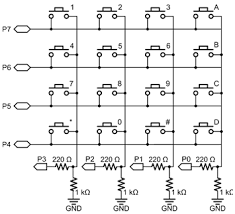
\includegraphics[scale=0.8]{fig/matrix_btn_4x4.png}
        \label{fig:matrix_btn_4x4}
    \end{figure}

    \answer{\textit{Programar!}}

  
    % ---- END OF FILE ----

\end{document}